\chapter{Testování}
\label{6-testovani}

\section{Letový kontrolér}
Testování algoritmu letového kontorléru bylo prováněno na vyrobené konstrukci. Konstrukce se skládá ze čtyř latěk, které tvoří rám. Uprostřed je upevněná kovová trubka, na které se pohybuje dron. Dron je pevně připevněn k trubce tak, aby pohyboval po obvodu trubky. Na stranách trubky jsou umístěny molitanové pruhy kvůli tlumení nárazu stojánku dronu.\\
Na konstrukci byla prováděna kalibrace PID regulátoru pro úhly pitch a roll. Kalibrace byla úspěšná při dostažení stabilizace dronu na trubce. Kalibrace byla prováděna pro úhel pitch, výsledky kalibrace se použijí i pro úhel roll.\\
Prvně byl zjištován koeficient pro proporcionální složku. Koeficient byl zvyšován do doby, než výkon vrtule dokázal dronu srovnat z nakloněné polohy do vodorovné. Derivační koeficient byl zvyšován do doby, kdy PID regulátor dokázal dronu stabilizovat ve vodorovné poloze. Integrační koeficient pouze doladil průběh PID regulátoru. Kalibrace PID regulátorů je závislá na parametrech motorů a konstrukci dronu, zjištěné koeficienty nebudou platit pro jiný dron.\\

\subsection{IMU filtry}
Pro použítí ovládání dronu byly uvažovány dva filtry Mahonyho a komplementární. Jednotlivé filtry byly testovány, jak obrazově tak i numericky.\\
Obrazově byla testována reakce na pohyb a ustálení polohy.
Po reakční stránce a ustálení  polohy byl lepší komplementární filtr. Vzhledem k jednoduchosti filtru, reakční doba IMU jednotky je minimální. Výsledky jsou patrné z grafů.\\
Numericky byl testován rozptyl střední hodnoty. Byla použita data po ustálení polohy v časovém intervalu čtyř minut. Výsledky byly rovnocené, oba filtry měli rozptyl střední hodnoty v řádů setin stupně.\\
Pro ovládání dronu je potřebná rychlá reakce IMU jednotky, proto byl použit komplementární filtr.\\

\begin{table}[]
		\centering
	
	\begin{tabular}{|l|l|l|}
		\hline
		\textbf{Úhel} & \textbf{Hodnota} & \textbf{Rozptyl} \\ \hline
		roll          & -0.730 $^\circ$  & 0.015 $^\circ$   \\ \hline
		roll          & -0.667 $^\circ$  & 0.014 $^\circ$   \\ \hline
		pitch         & 0.6390 $^\circ$  & 0.0030 $^\circ$  \\ \hline
		pitch         & 0.6880 $^\circ$  & 0.0030 $^\circ$  \\ \hline
	\end{tabular}
\caption{Komplementární filtr}
\end{table}

\begin{table}[]
			\centering
	\begin{tabular}{|l|l|l|}
		\hline
		\textbf{Úhel} & \textbf{Hodnota} & \textbf{Rozptyl} \\ \hline
		roll          & -0.739$^\circ$   & 0.015$^\circ$    \\ \hline
		roll          & -0.716 $^\circ$  & 0.013$^\circ$    \\ \hline
		pitch         & 0.7054 $^\circ$  & 0.0030$^\circ$   \\ \hline
		pitch         & 0.7132 $^\circ$  & 0.0030$^\circ$   \\ \hline
	\end{tabular}
\caption{Mahonyho filtr}
\end{table}

\begin{figure}[H]
	\centering
	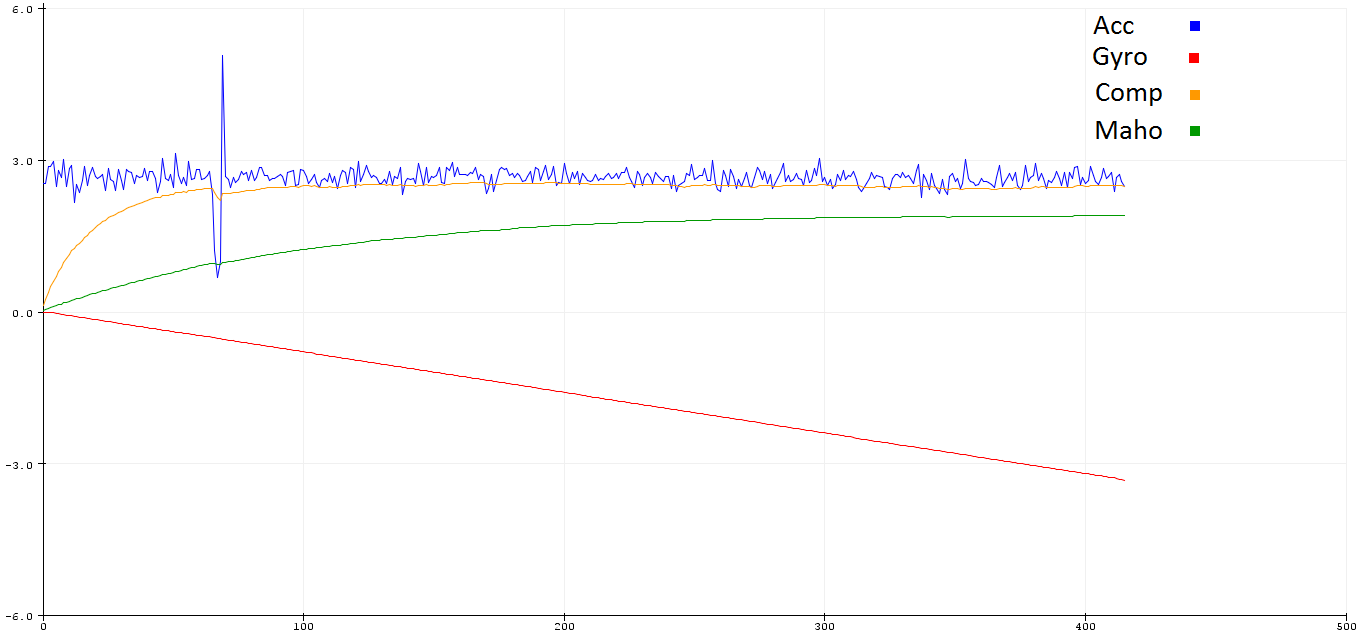
\includegraphics[width=14cm]{pictures/testRoll}
	\caption{Inicializace IMU}
\end{figure}

\begin{figure}[H]
	\centering
	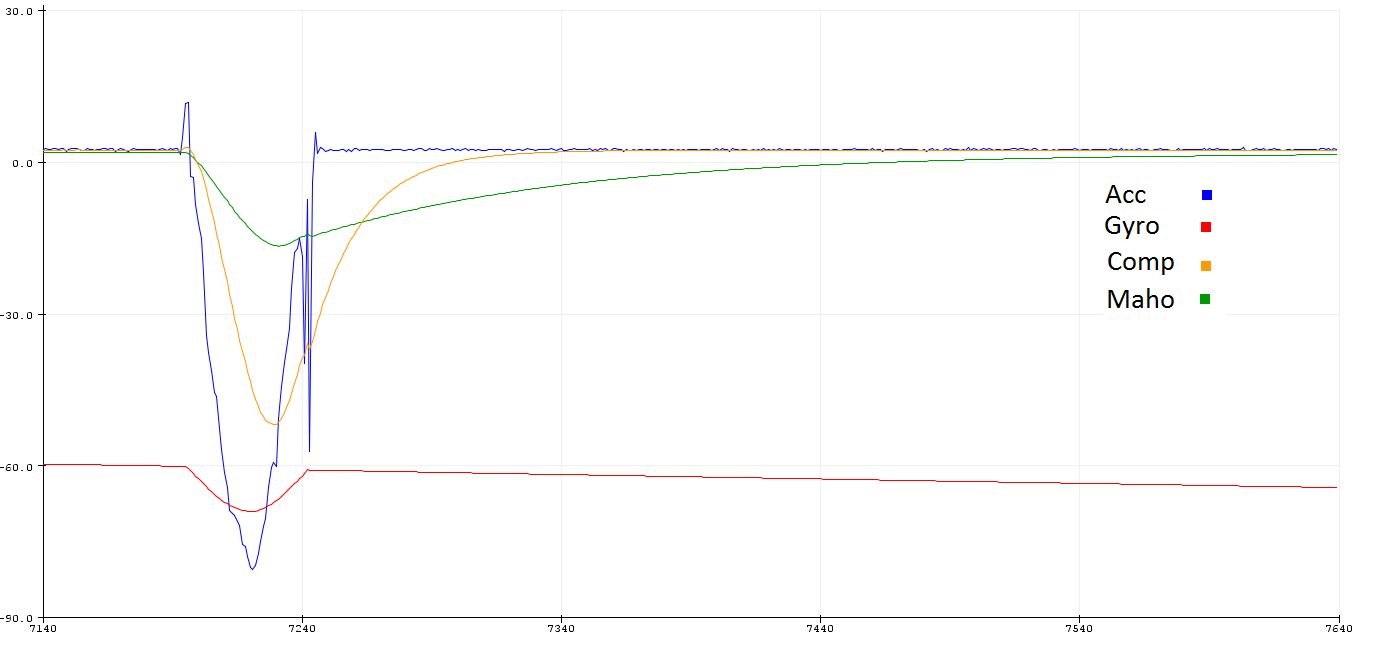
\includegraphics[width=14cm]{pictures/testRoll1}
	\caption{Náklon IMU jednotky}
\end{figure}

\begin{figure}[H]
	\centering
	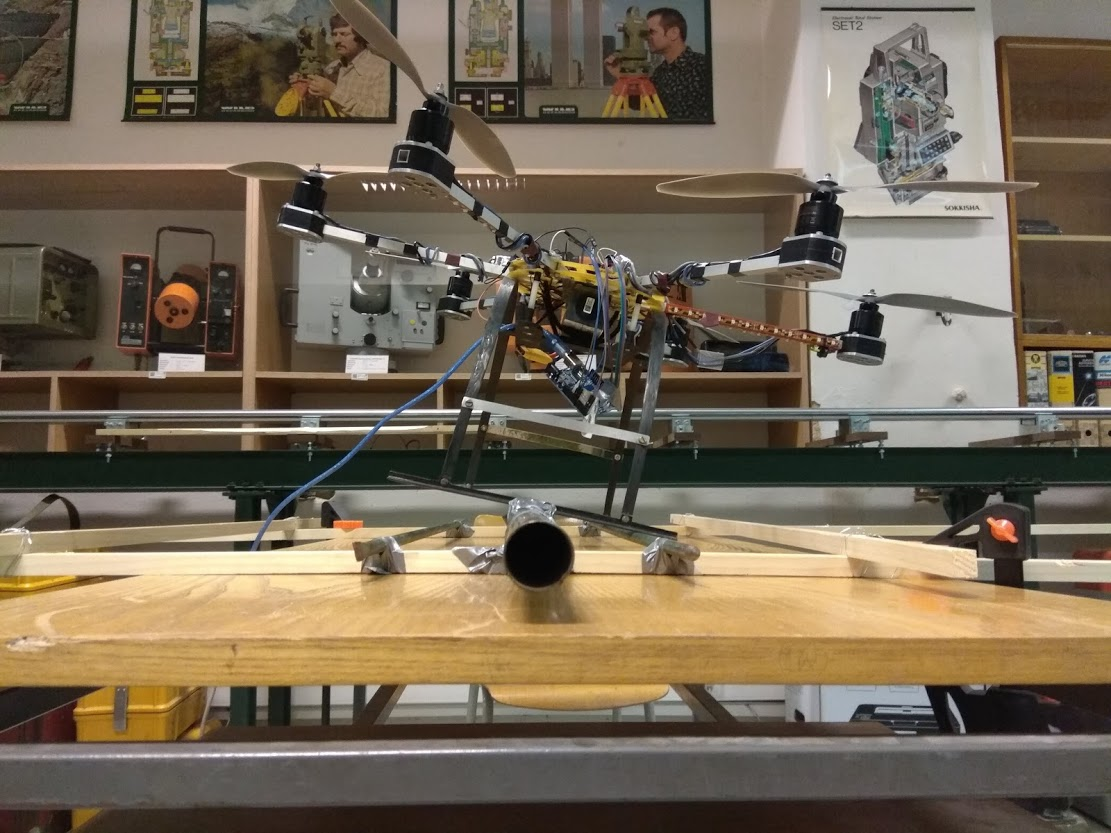
\includegraphics[width=10cm]{pictures/pidtest.jpg}
	\caption{Testování v konstrukci}
\end{figure}

\section{Překážový kontrolér}
Testovány byly laserové dálkoměry a komunikace mezi kontrolery. U laserových dálkoměrů byla ověřena přesnost měření a dosah. Překážkový kontrolér tedy dokáže upozornit o existující překážce ve vzálenosti 120 cm od konce ramene. Čas mezi jednotlivými měřením je menší než 1 ms.\\

\section{Navigační kontrolér}
Navigační kontrolér je ve fázi vývoje, zatím nebyl testován. Otestován byl pouze barometr, barometrem lze určit výška letu s přesností jednoho metru, pro přesnější měření se budou používat data z GNSS aparatury.\\

